\documentclass[12pt]{article}

\usepackage[paper=a4paper,left=25mm,right=25mm,top=25mm,bottom=25mm]{geometry}
\usepackage{url}
\usepackage{notoccite}
\usepackage{graphicx}
\usepackage{multirow}
\graphicspath{ {images/} }

\title{Projeto SMA, Rock Paper Scissors Lizard Spock}
\author{José Ferreira (53311), Afonso Seguro (57700), Catarina Lopes (57845)}

\begin{document}
	
	\maketitle
	
	\section*{Introdução}
    O projeto escolhido foi o “rock paper scissors lizard spock”, que consiste no jogo tradicional “rock paper scissor” com a adição de dois novos intervenientes, “lizard spock”. O jogo é constituído por 15 rondas, em que cada jogador tem 15 objetos (3 de cado tipo). A cada ronda os jogadores pedem o objeto utilizado na ronda. Ao longo do jogo, o jogador recebe 1 ponto por cada objeto do adversário que consegue atacar ou perde pontos quando o seu objeto é atacado.\\
    O objetivo deste trabalho é construir um sistema com vários agentes deliberativos, em que cada agente representa um jogador com tática diferente.\\
    Neste relatório, é mostrado como os agentes funcionam, o que inclui descrição da arquitetura do sistema e descrição da arquitetura interna dos agentes. No final, é demostrado o resultado da competição entre os diferentes jogadores.\\


	
	\section*{Arquitetura Geral}
    O sistema é composto por 7 agentes, um agente Mestre e seis 6 jogadores. O Mestre é responsável pela regulamentação da ronda, tornado assim, a peça central do sistema. Este agente não necessita de ser tão deliberativo como os restantes agentes jogadores (exceto o jogador\_Dummy), pois apenas tem de recolher as jogadas e calcular os pontos associados as estas. Os restantes jogadores são:
    
    \begin{itemize}
        \item Jogador Minor
        \item Jogador MinMax
        \item Jogado Prob
        \item Jogador All 1
        \item Jogador All 2
        \item Jogador Dummy
    \end{itemize}
    
    Inicialmente, pensou-se em utilizar o “Contract Network Protocol” para implementar o sistema descrito. No entanto, existiu a necessidade de utilizar vários behaviours, o que pareceu ser complicado implementar com o CN. Isto demonstrado nas classes Mestre\_CN e Jogador\_CN.\\
    
    A solução escolhida, passa pela criação de protocolo de comunicação, que se destacou pela sua simplicidade. Neste protocolo, o agente Mestre envia a cada jogadora as antigas jogadas e espera que estes respondam com a sua jogada para a ronda atual. Após receber a jogada de todos os jogadores, calcula os pontos consoante as jogadas. Este processo é repetido ao longo das 15 rondas.\\
    	
	\begin{figure}[h]
		\centering
		\includegraphics[width=0.80\textwidth]{arquiteturageral.eps}
		\caption{Arquitetura Geral}
		\label{fig:arquiteturageral}
	\end{figure}
	
	
    Como não existem jogadas anteriores na primeira ronda, o índice do jogador, isto é, a posição do jogador no array onde são enviadas as jogadas anteriores.\\
	
	
	\section*{Arquitetura interna dos agentes}
	
    Nesta secção vamos mostrar a arquitetura interna de cada agente, quais comportamentos os constituem, onde e como são calculados os planos consoante as crenças, os desejos e as intenções, e como tudo junto resulta na ação.\\
    Como já interpelado, vamos abordar os seguintes agentes:\\

    \begin{itemize}
        \item Jogador Mestre
        \item Jogador Minor
        \item Jogador MinMax
        \item Jogado Prob
        \item Jogador All 1
        \item Jogador All 2
        \item Jogador Dummy
    \end{itemize}
	
	
	\subsection*{Mestre}
    O mestre, como já referido, não é propriamente um agente deliberativo, pois não cria planos nem os altera consoante intenções ou desejos, no entanto também não é um agente reativo, pois as suas ações são previamente calculadas, guardando jogadas e calculando classificações.\\
    Este mesmo é constituído por 4 comportamentos (Behaviour), como mostrada na figura abaixo, sendo o Play Behaviour o mais importante. Todos os outros são auxiliares ao bom funcionamento do jogo, como a recolha de agentes (Ticket Behaviour) ou a capacidade de repetir vários jogos (Cyclic Behaviour).\\

    
    \begin{figure}[h]
		\centering
        \includegraphics[width=0.80\textwidth]{mestre.eps}
		\caption{Behaviours mestre}
		\label{fig:mestre}
	\end{figure}
	
    O Play Behaviour é a alma do jogo, pois é este comportamento que permite o desenrolar de um jogo, como demonstrado no algoritmo abaixo, este behaviour começa por enviar as jogadas anteriores, à exceção da primeira, em que envia o índice do jogador, para o mesmo saber quais as suas jogadas, depois fica à espera de todas as respostas, quando chega, calcula as classificações, e se chegar as 15 rondas, mostras as classificações.\\

	\begin{figure}[h]
		\centering
        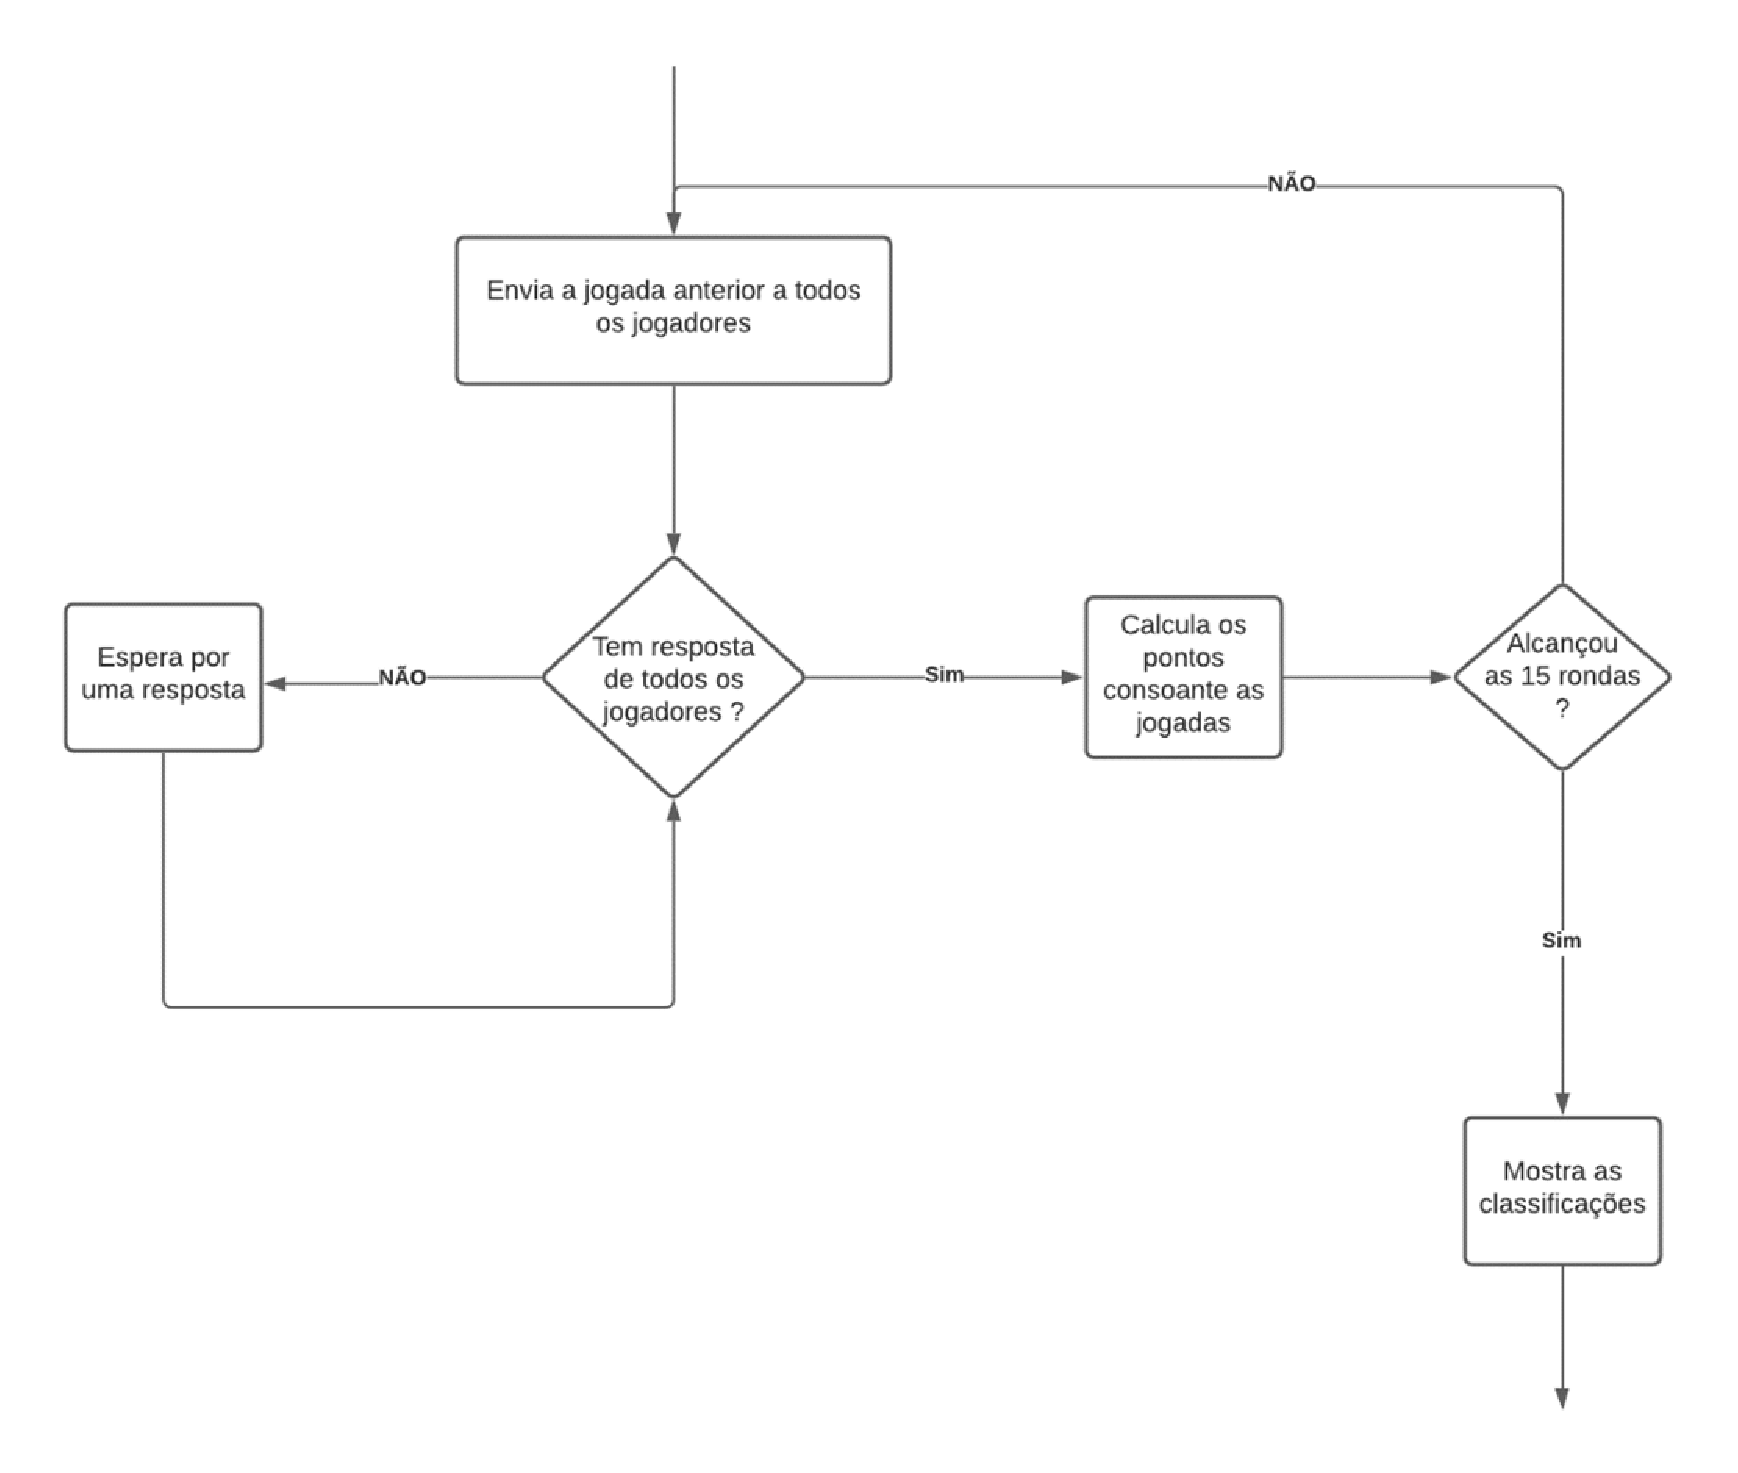
\includegraphics[width=0.80\textwidth]{mestrealg.eps}
		\caption{Play Behaviour mestre}
		\label{fig:mestrealg}
	\end{figure}
	

    O agente Mestre começa o jogo, quando recebe uma mensagem do tipo REQUEST de um agente Dummy. Esta mensagem faz com que o mestre execute o Play Behaviour e desta forma começar um jogo com os agentes que conhece.\\
	
	\subsection*{Jogador}
    Os jogadores em si, têm todos uma arquitetura interna idêntica, á exceção do jogador\_Dummy. Esta arquitetura é assente em três pilares:\\
	
	
	\begin{itemize}
        \item Crenças - Onde o jogador, recolhe todos os dados que sabe sobre o ambiente, ou seja, quais as mãos que lhe sobram, quais as mãos que sobram aos outros jogadores, quantas rondas faltam, etc…
        
        \item Desejos - O agente calcula quais as jogadas, ou sequência de jogadas, que pode realizar, ou seja, vários planos.
        
        \item Intenções - Este escolhe dos vários planos apresentados, quais os melhores, em prol do objetivo final de obter mais pontos.
    \end{itemize}

    
    A figura abaixo indica como é realizada a arquitetura base de cada agente jogador, consiste em 4 comportamentos (behaviours).\\
    O Cyclic behaviour, apenas espera por mensagens do mestre, nomeadamente as jogadas anteriores, e envia essas mesmas para o FSMBehaviour, a partir de uma fila.\\
    O FSM behaviour, é subdividido em 4 estados, as crenças, que abre a fila onde o Cyclic behaviour adiciona as jogadas feitas e calcula quais as mãos dos oponentes, tal como as mãos que sobram. Os desejos e as intenções variam consoante o tipo de agente, e o play, simplesmente envia uma mensagem para o mestre com uma jogada pré calculada.\\
    A partir daqui o que mais muda, é como é que cada agente gera os vários planos.\\

    \begin{figure}[h]
		\centering
        \includegraphics[width=0.80\textwidth]{jogador.eps}
		\caption{Behaviours jogador}
		\label{fig:jogador}
	\end{figure}
	
	\subsubsection*{Jogador MinMax}
    O jogador MinMax, implementa um algoritmo já há muito conhecido, este, consiste em calcular todas as possibilidades em cada ronda, sucessivamente ao longo de várias rondas até um limite imposto ou até se acabarem as mãos. Como tal, não é um tipo de jogador que possa ser muitas vezes utilizado, pois ao calcular todas as mãos durante vários níveis, quando mais jogadores existem no jogo, mais tempo demora a responder, sendo a complexidade temporal exponencial.\\
    Este agente, no estado de desejos, tenta criar vários planos, calculando, até um nível pré imposto, todas possíveis, e retornando o valor de calculo de maior número de pontos por cada jogada.\\
     Na intenção, pega em todas as jogadas possíveis apresentadas pelo estado de desejo, e verifica qual delas tem maior cotação, ou seja, qual a jogada que pode dar mais pontos a longo tempo. E de seguida é enviado para o estado “PLAY” que envia a jogada ao mestre.\\


	\subsubsection*{Jogador All1/All2}
    O jogador All, é bastante idêntico ao MinMax, no entanto não é tão complexo, apenas calcula o primeiro nível de profundidade. O que muda principalmente é como são escolhidos os planos, ou jogadas, que vão ser utilizados na próxima ronda. Tem duas versões (All\_1, All\_2).\\
    As crenças, são iguais ao modelo geral do jogador, apenas atualiza os seus dados consoante as jogadas realizadas pelos outros jogadores.\\
    Os desejos, como já referido, é idêntico ao MinMax, no entanto, apenas calcula todas as possibilidades na próxima ronda sucessiva, sendo atribuído a cotação em pontos de todos os casos possíveis.
    As intenções pegam em todos os casos possíveis, e nos pontos que cada um fornece e o cálculo da próxima jogada é onde os dois jogadores diferem.\\
    O jogador All\_1, soma todos os pontos, que por cada mão possível, ou seja, somas todos os pontos dos casos que foi jogado tesoura, ou outro, escolhendo no final, qual a jogada a ser feita consoante a mão que obtiver mais pontos.\\
    O jogador All\_2, realiza exatamente o mesmo, mas ao invés de somar os pontos por cada caso possível, soma 1 nos casos que obteve pontuação positiva e -1 nos de pontuação negativa.\\
    A grande diferença entre eles, é nos casos em que uma mão possa ganhar mais pontos no total de todos os casos possíveis, mas, no entanto, não quer dizer que ganhe a maioria dos casos, o jogador all\_1, opta pela mão que obteve mais pontos, e o jogador all\_2 opta pela mão que ganha mais casos. A passo de exemplo, imaginando que a mão tesoura obtém 10 pontos, mas apenas ganha 15 de 30 jogos possíveis, e a mão papel ganha 5 pontos, mas ganha 20 de 30 casos, o jogador All\_1 escolhe a mão tesoura e o All\_2 a mão papel.\\


	\subsubsection*{Jogador Prob}
    O jogador Prob, é dos que mais difere dos outros agentes, tando na criação de planos, como na escolha dos mesmos.\\
    Este jogador nas crenças, apenas atualiza as suas mãos possíveis, como as dos opoentes com as informações vinda do mestre.\\
    Nos desejos, é onde mais difere dos outros, pois este soma todas as mãos de todos os jogadores, ou seja, vê quantas tesouras é podem ainda ser jogadas, quantos papeis podem ser jogados e etc. Sendo que os que tiverem maior valor, é os que têm mais probabilidade de saírem pelos oponentes.\\
    Nas intenções, este pega em todas as mãos que ainda lhe sobram e compara com as mãos com maior probabilidade de sair, sendo atribuído uma cotação igual á quantidade de mãos que existem vezes 1 se ganhar, ou -1 se perder. No final, é tudo somado, e a mão que tiver maior cotação é enviada para o estado play para ser jogado.\\


	\subsubsection*{Jogador Minor}
    O jogador Minor, contem uma estratégia baseada na contagem de cartas. Ele contém 5 variáveis (inteiros), cada uma designada a cada tipo de objeto, todas inicializadas com o número total de cartas desse tipo que há em jogo.\\
    As crenças, são definidas pela simples adição de todas as jogadas realizadas até ao momento por todos os jogadores.\\
    Este jogador nos desejos, vê todas as cartas que saíram na ronda atual e desconta nas variáveis de cada objeto, fazendo assim com que seja contabilizado quantas cartas de cada tipo há em jogo.\\
    Nas intenções, o jogador vê qual o tipo de carta que existe menos e procura, a partir das cartas que tem na mão jogar contra essa carta. Como há sempre duas possibilidades de ganhar contra um tipo de carta, este jogador escolhe o tipo do qual ele tiver mais cartas. Caso ele não consiga jogar uma carta que ganhe contra a que existe menos, ele joga essa mesma carta e se nenhuma das opções anteriores for possível ele joga uma carta aleatoriamente.\\

	
	\subsubsection*{Jogador Dummy}
	O jogador Dummy não tem nem desejos nem intenções apenas responde com uma mão aleatória.\\
	
	
	\section*{Resultados, comparação de agentes}
    Nesta secção do relatório, vamos comparar todos os agentes, tanto em partidas de 1 vs 1 como em jogos com todos os elementos. No final realizamos uma pequena analise dos resultados e as conclusões retiradas.\\
	
	\subsection*{1 vs 1}
	
	\begin{center}
	    \begin{tabular}{ |p{4cm}|p{2cm}|p{2cm}|p{2cm}|p{4cm}|  }
	    \hline
	     Jogador/Partidas & 1ª & 2ª & 3ª & Vencedor Final \\\hline
         Dummy vs Dummy	& Segundo	& Segundo	& Segundo	& Dummy\\\hline
         Dummy vs Prob	& Primeiro	& Primeiro	& Primeiro	& Dummy\\\hline
         Dummy vs All2	& Primeiro	& Segundo	& Segundo	& All2\\\hline
         Dummy vs All1	& Primeiro	& Primeiro	& Primeiro	& Dummy\\\hline
         Dummy vs MinMax	& Primeiro	& Segundo	& Segundo	& MinMax\\\hline
         Dummy vs Minor	& Primeiro	& Primeiro	& Primeiro	& Dummy\\\hline
         Prob vs Prob	& Primeiro	& Primeiro	& Primeiro	& Prob\\\hline
         Prob vs All2	& Primeiro	& Primeiro	& Primeiro	& Prob\\\hline
         Prob vs All1	& Primeiro	& Primeiro	& Primeiro	& Prob\\\hline
         Prob vs MinMax	& Segundo	& Primeiro	& Segundo	& MinMax\\\hline
         Prob vs Minor	& Segundo	& Segundo	& Segundo	& Minor\\\hline
         All2 vs All2	& Primeiro	& Primeiro	& Primeiro	& All2\\\hline
         All2 vs All1	& Segundo	& Segundo	& Segundo	& All1\\\hline
         All2 vs MinMax	& Segundo	& Segundo	& Segundo	& MinMax\\\hline
         All2 vs Minor	& Segundo	& Segundo	& Primeiro	& Minor\\\hline
         All1 vs All1	& Primeiro	& Primeiro	& Primeiro	& All1\\\hline
         All1 vs MinMax	& Segundo	& Segundo	& Segundo	& MinMax\\\hline
         All1 vs Minor	& Segundo	& Segundo	& Segundo	& Minor\\\hline
         MinMax vs MinMax	& Segundo	& Segundo	& Segundo	& MinMax\\\hline
         MinMax vs Minor	& Segundo	& Primeiro	& Segundo	& Minor\\\hline
         Minor vs Minor	& Primeiro	& Segundo	& Primeiro	& Minor\\\hline
	    \end{tabular}
	\end{center}
	
    Na tabela acima, é apresentado as partidas entre todos os jogadores individualmente, sendo decidido após a vitoria em maioria de três jogos por partida. Consegue-se perceber que o jogador MinMax e o jogador Minor foram os que obtiveram melhores classificações, dando uma vantagem ao Minor que ganhou no confronto direto contra o jogador MinMax. De resto, de notar que o Dummy também teve um bom número de vitorias, que a tática de jogadas aleatórias acaba por ser melhor que algumas deliberativas.\\
	
	\subsection*{Todos vs Todos}
    Na disposição de vários contra vários, foi realizado 10 jogos de 15 rondas cada, com o âmbito de analisar qual o jogador que obteve mais vitorias.\\
    Devido ao tempo que alguns jogadores demoram a jogar, foi decidido utilizar apenas uma profundidade de 1 no jogador MinMax, isto relembrando que a complexidade temporal é exponencial consoante o número de jogadores, porque há mais casos possíveis de jogadas.\\

    
    
	\begin{center}
	    \begin{tabular}{ |p{1.5cm}|p{1.5cm}|p{1.5cm}|p{1.5cm}|p{1.5cm}|p{1.5cm}|p{1.5cm}|p{2cm}|  }
	    \hline
	    Jogo & All1	& All2	& Dummy & MinMax & Minor & Prob & Vencedor\\\hline
	    1	& -16	& -16	& 16	& 8	    & 0	    & 8	    & Dummy\\\hline
        2	& -3	& -3	& -6	& -5	& 1	    & 16	& Prob\\\hline
        3	& 1	    & 1	    & -21	& 0     & 4	    & 15	& Prob\\\hline
        4	& -12	& -12	& 9	    &10     & -4	& 9	    & MinMax\\\hline
        5	& 1	    & 1	    & -2	& 10	& 4	    & -14	& MinMax\\\hline
        6	& -4	& -4	& 1	    & -6	& 14	& -1	& Minor\\\hline
        7	& -10	& -10	& 3	    & 8	    & -3	& 12	& Prob\\\hline
        8	& -4	& -4	& -6	& 14	&-5	    & 5	    & MinMax\\\hline
        9	& -2	& -2	& -14	& 9	    & 1	    & 8	    & MinMax\\\hline
        10	& -3	& -3	& -6	& 14	&-5	    & 3	    & MinMax\\\hline
	    \end{tabular}
	\end{center}
	
	
	\begin{center}
	    \begin{tabular}{ |p{4cm}|p{1.5cm}|p{1.5cm}|p{1.5cm}|p{1.5cm}|p{1.5cm}|p{1.5cm}|  }
	    \hline
	    Jogador  & MinMax   & Prob  & Minor & Dummy & All1  & All2\\\hline
	    Nº de vitórias	& 5	    & 3	    & 1	    & 1	    & 0	    & 0\\\hline
        Média de pontos & 6.2   & 6.1   & 0.7	& -2.6	& -5.2	& -5.2\\\hline
	    \end{tabular}
	\end{center}
	
    Na primeira tabela apresentada, é demonstrado o resultado de 10 jogos, apresentando também o vencedor de cada. A primeira conclusão, foi a maioria de vitorias do algoritmo MinMax e Prob, pois estes são os que mais jogam em conta com as futuras jogadas, ou seja, os seus planos tendem a olhar para as rondas mais longínquas, não se preocupando apenas com a ronda jogada agora.\\
    A segunda tabela demostra a média de pontos ganhos no total, tal como o número de vitórias, percebe que os dois são proporcionalmente diretos, pois quanto maior a média de pontos, maior as vitórias.\\
    Outro jogador que sobressaio foi o jogador Prob, tendo apenas menos uma decima de diferença do MinMax, que tem um tanto de ironia, pois o MinMax tem mais parecenças com os jogadores All, e, no entanto, são os mais extremados da classificação final, mas tendo o jogador MinMax e Prob métodos tão diferentes, e classificações tão próximas.\\


	\section*{Conclusão}
    Com este trabalho podemos retirar várias conclusões, pela demonstração de uma arquitetura geral para a comunicação de vários agentes, às arquiteturas internas de cada jogador, e a criação de vários algoritmos aplicáveis a este jogo. Como tal, a partir dos resultados obtidos conseguimos perceber quais as arquiteturas que melhor se aplicam, como as crenças são fundamentais para fazer planos, pois é o que o agente conhece do ambiente, e como diferentes desejos e intenções afetam a ação final, de notar que aquelas com maior mira a rondas futuras tendem a ser melhores.\\
    Sendo o objetivo a construção de sistemas multiagentes na resolução de problemas complexos, o trabalho demonstra que se conseguiu atingir o objetivo a que estava proposto. Foi uma experiência bastante enriquecedora, não só a nível académico como também pessoal. Permitiu-nos também crescer como pessoas e adquirir qualidades de extrema importância no mundo da programação e conhecimentos até à data ainda não adquiridos ou consolidados\\


	
\end{document}